\documentclass[colorlinks=true, allcolors=blue]{article}
\usepackage{hyperref}
\usepackage{float}
\usepackage{verbatim}
\usepackage{placeins}    % for \FloatBarrier
\usepackage{setspace}    % to customize line spacing

% Drawing diagrams
\usepackage{tikz}
\usetikzlibrary{arrows.meta, positioning}

% Language setting
% Replace `english' with e.g. `spanish' to change the document language
\usepackage[english]{babel}

% Set page size and margins
% Replace `letterpaper' with `a4paper' for UK/EU standard size
\usepackage[letterpaper,top=2cm,bottom=2cm,left=3cm,right=3cm,marginparwidth=1.75cm]{geometry}

% Useful packages
\usepackage{amsmath}
\usepackage{graphicx}
\usepackage{caption}

% Removing Indents & setting line spaces
\setlength{\parindent}{0pt}
\setstretch{1.25}

% Title, Author, Problems/Date
\title{Computer Networks - Transport Layer}
\author{JJ McCauley \\ 4/20/25}
\date{Chapter 3's Problems: 3, 14, 27, 28, 36, 40}

\begin{document}
\maketitle

% Question 3
\setcounter{section}{2}
\section{UPD/TCP Checksum Calculation and Error Detection}
We are given three 8-bit bytes: \textbf{01010011}, \textbf{01100110}, and \textbf{01110100}. 

In order to calculate the 1's complement of these three 8-bit bytes, we must first \textit{add them together}. This will give us:
\[
01010011 + 01100110 + 01100110 = 10111001 + 01100110 =  \textbf{1} 00101101
\]
This gives us a 9-but number, but since we are limited to 8 bits, we must wrap around the carry the overflowed number.
\[
00101101 + 00000001 = 00101110
\]
This gives us the sum of the three 8-bit bytes. However, we are asked to find the 1's complement, so we can simply swap the binaries such that:
\[
\text{1's Complement = \textbf{11010001}}
\]
However, the arises the question- Why even take the 1's complement in the first place? Ultimately, UCP/TCP uses 1's complement of the sum because it makes \textbf{error detection easier}. \\

Using the 1's complement allows the receiver to check for errors by \textbf{adding all the received data, including the checksum}. If no errors occurred, the result of the sum should be all 1s, which helps with detecting whether a bit was flipped and detecting other errors that could cancel out with 0s. \textbf{If the result is not all 1s, an error is detected}. \\

Therefore, \textbf{1 bit errors will never go undetected}. \textbf{2-bit errors}, however, \textbf{can sometimes go undetected} as two bits could flip in a way that cancels each other out and make the sum still appear valid.

% Question 14
\setcounter{section}{13}
\section{NAK-Only vs ACK-Based Protocol Efficiency}
We are asked to evaluate NAK-only and ACK-Based protocols for two scenarios: a sender that sends data only infrequently, and a sender that has a lot of data to send and the end-to-end connection experiences few losses.
\subsection{Sending Data Infrequently}
In this scenario, a \textbf{NAK-only protocol} would be preferable. This is because, in this scenario, the sender only sends rarely with data only being sent occasionally, not continuously. Since data is sent infrequently, a NAK-only protocol would send messages only when there is an error, reducing overhead with fewer general control messages and less bandwidth wasted. 
\subsection{Sending Data Frequently with Few Losses}
In this scenario, a \textbf{ACK-based protocol} would be preferable. This scenario presents the sending sending lots of data (high throughput) and few losses (reliable channel). The ACK-based protocol provides feedback with every packet, which would allow for the sender to detect issues sooner if an ACK is missing (especially important with continuous data) and would allow the sender to implement flow and congestion control more effectively. This offers better control and synchronization, improving error recovery and performance.

% Question 27
\setcounter{section}{26}
\section{TCP Segment Ordering \& Acknowledgment Behavior}
We are given a scenario where host A and B are communicating over a TCP connection, with Host B receiving from A all bytes up to byte 126. Host A then sends Host B two segments back-to-back, with the first segment containing 80 bytes and the second containing 40 bytes. In the first segment, the sequence number is 127, the source port number is 302, and the destination port number is 80. Host B sends an acknowledgment whenever it receives a segment from Host A.
\subsection{Sequence \& Port Numbers of the Second Segment}
In order to retrieve the \textit{sequence number}, we must determine the next byte expected (which will be the sequence number). Since we are given the size of the first segment (40 bytes) and the sequence number (127), we can simply add them together such that:
\[
127 + 80 = \textbf{207}
\]
Which will be the sequence number of the second segment. \\

Since we are using TCP, we know that the ports will not change, since everything is transferred within the same connection. Therefore, for the second segment, the \textbf{source port is 302} and the \textbf{destination port is 80}, the same as the first segment.
\subsection{ACK When First Segment Arrives Before Second}
Since TCP acknowledgments are cumulative, the ACK number is the next expected byte. Through the calculations previously executed, we therefore know that the \textbf{ arc number is 207}. \\

Unlike the previous section, ACKs flip the source and destination ports because the reply is going back from Host B to Host A. Therefore, the \textbf{Source Port is 80}, while the \textbf{Destination port is 302}.
\subsection{ACK When Second Segment Arrives Before First}
In this case, Host B has only received up to byte 126 so far. TCP delivers data in order and uses cumulative ACKs, so it will refuse to acknowledge byte 207 (as calculated above) until it receives everything up to byte 206. Therefore, Host B will ignore the out-of-order segment, and \textbf{it will still ACK 127} as it is waiting on the bytes from 127 to 206.
\subsection{TCP Timing Diagram with Lost ACK and Timeout}

% Thank you chatGPT for this wonderful graph
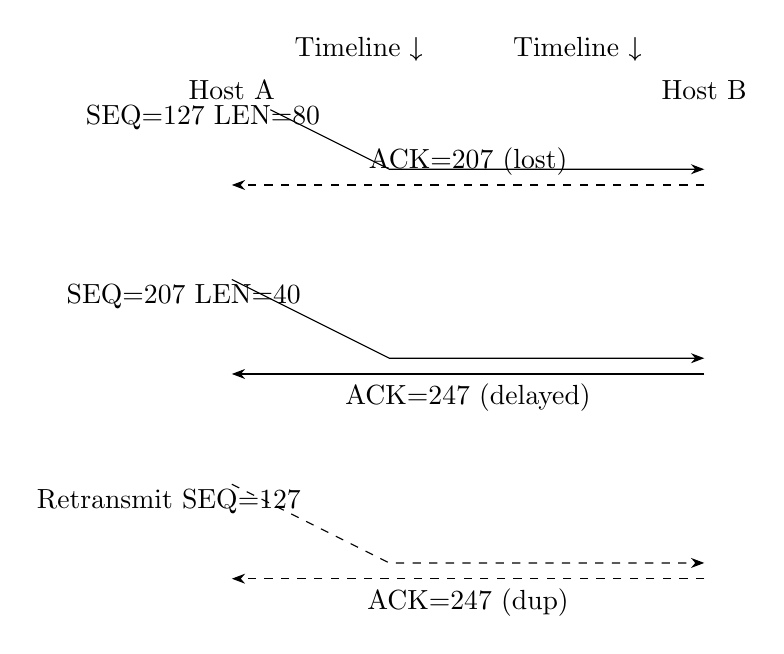
\begin{tikzpicture}[>=Stealth, node distance=1.8cm and 2.5cm]

% Nodes for Host A and B
\node (A) at (0,0) {Host A};
\node (B) at (6,0) {Host B};

% Arrows: SEQ=127, LEN=80
\draw[->] (A) -- ++(2,-1) node[midway, above left] {SEQ=127 \\ \space LEN=80} -- ++(4,0);

% ACK=207 (lost)
\draw[dashed,->] (B) ++(0,-1.2) -- ++(-6,0) node[midway, above] {ACK=207 (lost)};

% Arrows: SEQ=207, LEN=40
\draw[->] (A) ++(0,-2.4) -- ++(2,-1) node[midway, above left] {SEQ=207 \\ \space LEN=40} -- ++(4,0);

% ACK=247 (arrives late)
\draw[->] (B) ++(0,-3.6) -- ++(-6,0) node[midway, below] {ACK=247 (delayed)};

% Timeout and retransmission of SEQ=127
\draw[->, dashed] (A) ++(0,-5) -- ++(2,-1) node[midway, above left] {Retransmit \\ \space SEQ=127} -- ++(4,0);

% Optional duplicate ACK (if B responds again)
\draw[->, dashed] (B) ++(0,-6.2) -- ++(-6,0) node[midway, below] {ACK=247 (dup)};

% Labels for vertical flow
\node[align=center, above right] at (A.north east) {Timeline ↓};
\node[align=center, above left] at (B.north west) {Timeline ↓};

\end{tikzpicture}

% Question 28
\section{TCP Flow Control with Mismatched Send \& Receive Rates}
In this scenario, we are given a link speed (100 Mbps), Host A send rate (Max 120 Mbps), and Host B receive rate (Max 50 Mbps). Clearly, we can see that \textbf{Host B's receive rate} will \textbf{bottleneck the entire TCP connection}. \\
This is due to TCP's \textbf{flow control}, which ensures that the receiving host isn't overwhelmed. TCP uses a receiving window to tell the sender how much buffer space is available from the receiver. When the sender (Host A with a faster sending and link rate) starts sending data into Host B's receive buffer, it will dynamically adjust the receiving window until it becomes 0 when Host B's buffer becomes full. This causes Host A to pause transmission until the contents of the buffer are processed, decreasing any packet loss from Host A overwhelming Host B with data.

% Question 36
\setcounter{section}{35}
\section{Why TCP Waits for Three Duplicate ACKs}
The designs of TCP likely implemented waiting for three duplicate ACKs before retransmitting due to the fact that packets could just be \textbf{out of order}. Networks may not always receive/deliver packets in order (which is normal), so retransmitting after a single duplicate ACK could waste bandwidth and cause more congestion. 

For example, lets say Host B is receiving packets from Host A. Host B receives bytes 1-100, sending an ACK of 101. It is now expecting a segment starting with byte 101, however it may receive bytes 201-300. This would still send an ACK of 101, although it still received bytes, just out of order. It is only when Host A receives 3 identical Acks that it assumes that Host B needs the segment starting with 101, so it will resend that segment. If it were to have sent it after the first ACK, it could cause congestion, as it is expected for segments to occasionally be send out of order.

% Question 40
\setcounter{section}{39}
\section{TCP Reno Congestion Window Behavior}
Given a diagram of TCP window size as a function of time, we are asked the following questions:

\subsection{Intervals of TCP Slow Start}
TCP slow start is the phase where TCP doubles the congestion window each RTT, continuing until it hits the slow-start threshold. Within the diagram, we can see that the congestion window doubles every round until about transmission round 6, which it hits the slow-start threshold and starts balancing out. Therefore, \textbf{TCP slow start is operating from round 0 to around round 6} and again from \textbf{about round 23 to 26}, where we can start to see the same pattern.

\subsection{Intervals of TCP Congestion Avoidance}
TCP congestion avoidance is the phase where the congestion window increases linearly, starting after slow start ends and once the slow-start threshold is reached.  Within the diagram, we can see that a linear movement (and \textbf{the TCP congestion avoidance phase}) occurs \textbf{from round 6 to about 16}, then again from \textbf{about round 17 to 22}.

\subsection{16th Transmission Round}
The sharp dip around round 16 can be attributed to either \textit{three duplicate ACKs} or \textit{timeout}. When three duplicate ACKs occur, it assumes that a packet was lost, but the network is still delivering other packets. This is not treated as severe congestion, and therefore the congestion window size decreases sharply but does not reach 0 (typically about halves). This is what occurs during round 16, with the congestion window size decreasing from around 42 to 24, then picking back up with the TCP congestion avoidance phase. Therefore, \textbf{round 16} can \textbf{be attributed to three duplicate ACKs}.

\subsection{22nd Transmission Round}
Similarly to the previous question, this dip can be attributed to either \textit{three duplicate ACKs} or \textit{timeout}. In TCP, timeouts are considered a serious sign of congestion, with the congestion window sharply cutting down to about 1 (since no packets could be getting through at all). Then, the congestion window will start exponentially picking back up again with the slow start phase, attempting to maximize the amount of packets sent after the sharp decline. This behavior is observed in \textbf{round 22}, and can therefore \textbf{be attributed to timeout}.

\subsection{Initial Value of Slow Start Threshold}
The slow start threshold is the value that determines when TCP should switch from \textit{slow start} to \textit{congestion avoidance} phase. Observing the diagram, we can see that this behavior is observed around \textbf{32 segments} (sshtresh size), which is where the line behavior switches from exponential (\textit{slow start}) to linear (\textit{congestion avoidance phase}).

\subsection{Value of Slow Start Threshold at the 18th Transmission Round}
Around round 16, there is a sharp decline in the congestion window size, which we earlier attributed to \textit{3 duplicate ACKs}. When this occurs, the congestion window size typically halves, which is observed in the diagram. Looking closer, we can see that the \textbf{congestion window size at round 18} is around \textbf{25 segments}.

\subsection{Value of Slow Start Threshold at the 24th Transmission Round}
Around round 22, there is a very sharp decline in the congestion window size, which we earlier attributed to \textit{timeout}. When this occurs, the window size typically drops to 1, due to significant congestion being detected. This is observed in the diagram, with looking closer revealing the \textbf{congestion window size at round 22}, after shortly recovering in the slow start phase, is around \textbf{2 segments}.

\subsection{Transmission Round of 70th Segment Sent}
To determine what round the 70th segment is sent, we can simply count and sum up the number of segments found at each round.
\begin{table}[H]
\centering
\begin{tabular}{|c|c|c|}
\hline
\textbf{Round} & \textbf{Segments Sent} & \textbf{Cumulative Segments Sent} \\
\hline
1 & 1 & 1 \\
2 & 2 & 3 \\
3 & 4 & 7 \\
4 & 8 & 15 \\
5 & 16 & 31 \\
6 & 32 & 63 \\
7 & 33 & 96 \\
\hline
\end{tabular}
\caption{Transmission Rounds vs Cumulative Segments Sent}
\end{table}
As we can see, the \textbf{70th segment} is sent during \textbf{round 7}.

\subsection{Values of Congestion Window Size and ssthresh after Three Duplicate Acks at Round 26}
If we were to assume that packet loss is detected after the 26th round by \textit{three duplicate ACKs}, we can take the strategy mentioned above of \textit{halving} the congestion window size at round 26. We see that the \textbf{congestion window size} is 12 at round 26, with 12/2 being \textbf{6 segments after round 26}. Additionally, we know that the slow start threshold will be the same after this, with the congestion window entering the \textit{TCP Congestion Avoidance phase} after three duplicate ACKs are detected. Therefore, the \textbf{slow start threshold} would equal the congestion window size, being \textbf{6 segments}.

\subsection{Values of Congestion Window Size and ssthresh after Three Duplicate Acks at Round 19, assuming TCP Tahoe}
TCP Tahoe acts similarly to TCP Reno, however it treats \textit{three duplicate ACKs} as if it was a \textit{timeout}. Therefore, it will half the slow start threshold, and reset the congestion window size. Therefore, at round 16 (where the three duplicate ACKs occured, as previously discussed), the \textbf{slow start theshold} is set to 42/2=\textbf{21}, which will remain the same at round 19. Then, with a congestion window of size of 1 at round 16, it will double 3 times by the time it reaches round 19, following the order of 1-\>2-\>4-\>8. Therefore, the \textbf{congestion window size} at round 19, assuming three duplicate ACKs and TCP Tahoe, would be \textbf{8 segments}.

\subsection{Total Packets Sent after Timeout at Round 22, assuming TCP Tahoe}
In order to calculate the total packets sent from the 17th to 22nd round (inclusive), we must firstly remember the behavior observed in the last question. At round 16, the congestion window drops to 1, and the ssthresh is set to 21. Using this information, we can add all packets from round 17 to 22, remembering that the slow start phase is currently in session until it reaches the short start threshold.
\begin{table}[H]
\centering
\begin{tabular}{|c|c|c|}
\hline
\textbf{Round} & \textbf{Segments Sent} & \textbf{Cumulative Segments Sent} \\
\hline
17 & 1 & 1 \\
18 & 2 & 3 \\
19 & 4 & 7 \\
20 & 8 & 15 \\
21 & 16 & 31 \\
22 & 21 & 52 \\
\hline
\end{tabular}
\caption{Transmission Rounds vs Cumulative Segments Sent}
\end{table}
Therefore, \textbf{TCP Tahoe} would send \textbf{52 packets from rounds 17-22}. 

\clearpage  % Ensure that images successfully load in
\end{document}
